


\tikzset{every picture/.style={line width=0.75pt}} %set default line width to 0.75pt        

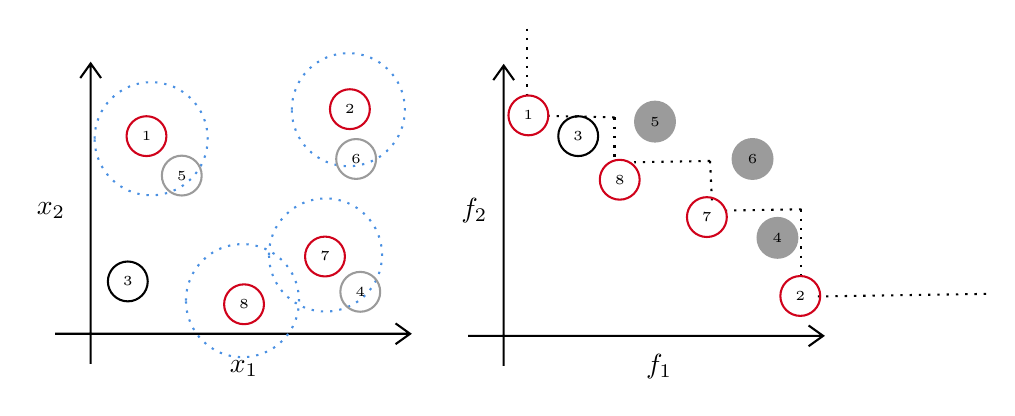
\begin{tikzpicture}[x=0.75pt,y=0.75pt,yscale=-1,xscale=1]
%uncomment if require: \path (0,340.9375); %set diagram left start at 0, and has height of 340.9375

%Shape: Circle [id:dp3061612047883613] 
\draw  [color={rgb, 255:red, 74; green, 144; blue, 226 }  ,draw opacity=1 ][dash pattern={on 0.84pt off 2.51pt}] (69,106.25) .. controls (69,91.2) and (81.2,79) .. (96.25,79) .. controls (111.3,79) and (123.5,91.2) .. (123.5,106.25) .. controls (123.5,121.3) and (111.3,133.5) .. (96.25,133.5) .. controls (81.2,133.5) and (69,121.3) .. (69,106.25) -- cycle ;
%Shape: Axis 2D [id:dp3645341276574614] 
\draw  (50,200.22) -- (221,200.22)(67.1,70) -- (67.1,214.69) (214,195.22) -- (221,200.22) -- (214,205.22) (62.1,77) -- (67.1,70) -- (72.1,77)  ;
%Shape: Axis 2D [id:dp14963900792703488] 
\draw  (249,201.22) -- (420,201.22)(266.1,71) -- (266.1,215.69) (413,196.22) -- (420,201.22) -- (413,206.22) (261.1,78) -- (266.1,71) -- (271.1,78)  ;
%Shape: Circle [id:dp4297581821087293] 
\draw  [color={rgb, 255:red, 74; green, 144; blue, 226 }  ,draw opacity=1 ][dash pattern={on 0.84pt off 2.51pt}] (164,92.25) .. controls (164,77.2) and (176.2,65) .. (191.25,65) .. controls (206.3,65) and (218.5,77.2) .. (218.5,92.25) .. controls (218.5,107.3) and (206.3,119.5) .. (191.25,119.5) .. controls (176.2,119.5) and (164,107.3) .. (164,92.25) -- cycle ;
%Straight Lines [id:da8256937375790945] 
\draw  [dash pattern={on 0.84pt off 2.51pt}]  (277.5,53.24) -- (277.5,85.24) ;


%Straight Lines [id:da017532966868774924] 
\draw  [dash pattern={on 0.84pt off 2.51pt}]  (409.5,140.24) -- (409.5,172.24) ;


%Straight Lines [id:da6557874814370408] 
\draw  [dash pattern={on 0.84pt off 2.51pt}]  (319.5,95.96) -- (287.5,95.24) ;


%Straight Lines [id:da3174724210407276] 
\draw  [dash pattern={on 0.84pt off 2.51pt}]  (498.5,181) -- (417.5,182.24) ;


%Straight Lines [id:da5438812387908785] 
\draw  [dash pattern={on 0.84pt off 2.51pt}]  (365.5,116.96) -- (366.5,137.24) ;


%Straight Lines [id:da4833984925117387] 
\draw  [dash pattern={on 0.84pt off 2.51pt}]  (409.5,140.24) -- (373,140.86) ;


%Shape: Circle [id:dp40124369257922843] 
\draw  [color={rgb, 255:red, 74; green, 144; blue, 226 }  ,draw opacity=1 ][dash pattern={on 0.84pt off 2.51pt}] (153,162.25) .. controls (153,147.2) and (165.2,135) .. (180.25,135) .. controls (195.3,135) and (207.5,147.2) .. (207.5,162.25) .. controls (207.5,177.3) and (195.3,189.5) .. (180.25,189.5) .. controls (165.2,189.5) and (153,177.3) .. (153,162.25) -- cycle ;
%Straight Lines [id:da24170189870934] 
\draw  [dash pattern={on 0.84pt off 2.51pt}]  (319.5,95.96) -- (319.5,114.96) ;


%Straight Lines [id:da06647806614736962] 
\draw  [dash pattern={on 0.84pt off 2.51pt}]  (365.5,116.96) -- (329,117.58) ;


%Shape: Circle [id:dp30757432980400146] 
\draw  [color={rgb, 255:red, 74; green, 144; blue, 226 }  ,draw opacity=1 ][dash pattern={on 0.84pt off 2.51pt}] (113,184.25) .. controls (113,169.2) and (125.2,157) .. (140.25,157) .. controls (155.3,157) and (167.5,169.2) .. (167.5,184.25) .. controls (167.5,199.3) and (155.3,211.5) .. (140.25,211.5) .. controls (125.2,211.5) and (113,199.3) .. (113,184.25) -- cycle ;

% Text Node
\draw  [color={rgb, 255:red, 208; green, 2; blue, 27 }  ,draw opacity=1 ]  (94, 105) circle [x radius= 9.6, y radius= 9.6]   ;
\draw (94,105) node  [font=\tiny] [align=left] {1};
% Text Node
\draw  [color={rgb, 255:red, 155; green, 155; blue, 155 }  ,draw opacity=1 ]  (111, 124) circle [x radius= 9.6, y radius= 9.6]   ;
\draw (111,124) node  [font=\tiny] [align=left] {5};
% Text Node
\draw  [color={rgb, 255:red, 208; green, 2; blue, 27 }  ,draw opacity=1 ]  (192, 92) circle [x radius= 9.6, y radius= 9.6]   ;
\draw (192,92) node  [font=\tiny] [align=left] {2};
% Text Node
\draw  [color={rgb, 255:red, 155; green, 155; blue, 155 }  ,draw opacity=1 ]  (195, 116) circle [x radius= 9.6, y radius= 9.6]   ;
\draw (195,116) node  [font=\tiny] [align=left] {6};
% Text Node
\draw  [color={rgb, 255:red, 208; green, 2; blue, 27 }  ,draw opacity=1 ]  (180, 163) circle [x radius= 9.6, y radius= 9.6]   ;
\draw (180,163) node  [font=\tiny] [align=left] {7};
% Text Node
\draw  [color={rgb, 255:red, 155; green, 155; blue, 155 }  ,draw opacity=1 ]  (197, 180) circle [x radius= 9.6, y radius= 9.6]   ;
\draw (197,180) node  [font=\tiny] [align=left] {4};
% Text Node
\draw  [color={rgb, 255:red, 208; green, 2; blue, 27 }  ,draw opacity=1 ]  (141, 186) circle [x radius= 9.6, y radius= 9.6]   ;
\draw (141,186) node  [font=\tiny] [align=left] {8};
% Text Node
\draw    (85, 175) circle [x radius= 9.6, y radius= 9.6]   ;
\draw (85,175) node  [font=\tiny] [align=left] {3};
% Text Node
\draw  [color={rgb, 255:red, 208; green, 2; blue, 27 }  ,draw opacity=1 ]  (278, 95) circle [x radius= 9.6, y radius= 9.6]   ;
\draw (278,95) node  [font=\tiny] [align=left] {1};
% Text Node
\draw  [color={rgb, 255:red, 155; green, 155; blue, 155 }  ,draw opacity=1 ][fill={rgb, 255:red, 155; green, 155; blue, 155 }  ,fill opacity=1 ]  (339, 98) circle [x radius= 9.6, y radius= 9.6]   ;
\draw (339,98) node  [font=\tiny] [align=left] {5};
% Text Node
\draw  [color={rgb, 255:red, 208; green, 2; blue, 27 }  ,draw opacity=1 ]  (409, 182) circle [x radius= 9.6, y radius= 9.6]   ;
\draw (409,182) node  [font=\tiny] [align=left] {2};
% Text Node
\draw  [color={rgb, 255:red, 155; green, 155; blue, 155 }  ,draw opacity=1 ][fill={rgb, 255:red, 155; green, 155; blue, 155 }  ,fill opacity=1 ]  (386, 116) circle [x radius= 9.6, y radius= 9.6]   ;
\draw (386,116) node  [font=\tiny] [align=left] {6};
% Text Node
\draw  [color={rgb, 255:red, 208; green, 2; blue, 27 }  ,draw opacity=1 ]  (364, 144) circle [x radius= 9.6, y radius= 9.6]   ;
\draw (364,144) node  [font=\tiny] [align=left] {7};
% Text Node
\draw  [color={rgb, 255:red, 155; green, 155; blue, 155 }  ,draw opacity=1 ][fill={rgb, 255:red, 155; green, 155; blue, 155 }  ,fill opacity=1 ]  (398, 154) circle [x radius= 9.6, y radius= 9.6]   ;
\draw (398,154) node  [font=\tiny] [align=left] {4};
% Text Node
\draw  [color={rgb, 255:red, 208; green, 2; blue, 27 }  ,draw opacity=1 ]  (322, 126) circle [x radius= 9.6, y radius= 9.6]   ;
\draw (322,126) node  [font=\tiny] [align=left] {8};
% Text Node
\draw    (302, 105) circle [x radius= 9.6, y radius= 9.6]   ;
\draw (302,105) node  [font=\tiny] [align=left] {3};
% Text Node
\draw (141,217) node    {$x_{1}$};
% Text Node
\draw (48,141) node    {$x_{2}$};
% Text Node
\draw (341,216) node    {$f_{1}$};
% Text Node
\draw (252,141) node    {$f_{2}$};


\end{tikzpicture}
